\chapter{Разработка методики обучения и дообучения физически информированной нейросетевой системы}
\label{ch:3}


% =========================================================
\section{Общая архитектура рассматриваемых нейронных сетей}
\label{sec:common_arch}
% =========================================================


В данной работе рассматриваются следующие нейронные сети:
\begin{enumerate}
	\item Предлагаемая в данной работе \textbf{физически информированная} нейронная сеть на основе последовательностей
	с селективными пространствами состояний с динамическим функционалом потерь.
	Динамический функционал основывается на законе тяги несущих винтов.
	Кратко обозначим как \textbf{ФИ НС-ПСПС}.
	\item Нейронная сеть на основе последовательностей с селективными
	пространствами состояний, учитывающая динамические ограничения платформы
	по внутренним состояниям системы, без учёта оборотов
	двигателей, ранее предложенная авторами в работе~\cite{Sidorenko2026}.
	Кратко обозначим как \textbf{ДИ НС-ПСПС}.
	\item Нейронная сеть на основе последовательностей с селективными
	пространствами состояний с базовым функционалом потерь $\mathcal{L}_{traj}$,
	содержащим только целевую ошибку по траектории; блок физических ограничений
	отсутствует. Кратко обозначим как \textbf{НС-ПСПС}
	Кратко обозначим как \textbf{базовая нейронная сеть}.
	\item Нейронная сеть на основе механизма внимания, включённая в сравнение
	как представитель альтернативного класса архитектур.
	В работе обозначается как \textbf{Transformer}.
\end{enumerate}

Обобщённая схема всех четырёх архитектур представлена на
рисунке~\ref{fig:compare}.
На схеме показаны входной вектор, ядро, выходной вектор и функционал потерь
для каждой из моделей.
Ключевые различия состоят в следующем.
Transformer использует ядро на основе механизма внимания и не включает
физических ограничений.
Базовая нейронная сеть использует ядро Mamba и базовый функционал
$\mathcal{L}_{traj}$, который является общей частью всех трёх НС на основе
пространственно-временной модели состояния.
Обобщённая нейронная сеть дополняет базовый функционал регуляризатором по
внутренним состояниям системы, не зависящим от оборотов.
Предлагаемая нейронная сеть дополнительно принимает на вход телеметрию
оборотов~$\mathbf{n}_t$ и включает физический регуляризатор, явно основанный
на законе тяги~\eqref{eq:thrust}, вычисляемый непосредственно из~$n_i$.

\begin{figure}
	\centering
	\resizebox{0.8\linewidth}{!}{% ================================================
% fig-compare.tex
% ================================================
\tikzset{
  cmp/inp/.style={
    rectangle, rounded corners=2pt,
    fill=blue!15, draw=blue!55, line width=0.7pt,
    font=\scriptsize\bfseries, align=center,
    minimum width=1.55cm, minimum height=0.9cm},
  cmp/rpm/.style={
    rectangle, rounded corners=2pt,
    fill=blue!35, draw=blue!70, line width=0.7pt,
    font=\scriptsize\bfseries, align=center,
    minimum width=1.55cm, minimum height=0.5cm},
  cmp/emb/.style={
    rectangle, rounded corners=2pt,
    fill=green!18, draw=green!55!black, line width=0.7pt,
    font=\scriptsize\bfseries, align=center,
    minimum width=1.2cm, minimum height=0.9cm},
  cmp/mamba/.style={
    rectangle, rounded corners=2pt,
    fill=yellow!30, draw=orange!65, line width=0.7pt,
    font=\scriptsize\bfseries, align=center,
    minimum width=1.55cm, minimum height=0.9cm},
  cmp/attn/.style={
    rectangle, rounded corners=2pt,
    fill=purple!15, draw=purple!55, line width=0.7pt,
    font=\scriptsize\bfseries, align=center,
    minimum width=1.55cm, minimum height=0.9cm},
  cmp/out/.style={
    rectangle, rounded corners=2pt,
    fill=orange!20, draw=orange!65, line width=0.7pt,
    font=\scriptsize\bfseries, align=center,
    minimum width=1.35cm, minimum height=0.9cm},
  cmp/loss/.style={
    rectangle, rounded corners=2pt,
    fill=gray!10, draw=gray!50, line width=0.7pt,
    font=\scriptsize\bfseries, align=center,
    minimum width=1.6cm, minimum height=0.9cm},
  cmp/phy/.style={
    rectangle, rounded corners=2pt,
    fill=red!12, draw=red!60, line width=0.8pt,
    font=\scriptsize\bfseries, align=center,
    minimum width=1.6cm, minimum height=0.7cm},
  cmp/physloss/.style={
    rectangle, rounded corners=2pt,
    fill=red!12, draw=red!60, line width=0.8pt,
    font=\scriptsize\bfseries, align=center,
    minimum width=1.6cm, minimum height=0.9cm},
  arr/.style={-{Stealth[length=3pt,width=2.5pt]},
    line width=0.7pt, color=gray!60},
  rarr/.style={-{Stealth[length=3pt,width=2.5pt]},
    line width=0.8pt, color=red!60},
  rdarr/.style={-{Stealth[length=3pt,width=2.5pt]},
    line width=0.8pt, color=red!60, dashed},
}

\usetikzlibrary{fit, calc}

\begin{tikzpicture}[every node/.style={font=\small}]

% ── заголовки столбцов ──
\node[font=\scriptsize\bfseries, text=gray!70] at (2.4,  0.62) {Вход};
\node[font=\scriptsize\bfseries, text=gray!70] at (4.9,  0.62) {Embed};
\node[font=\scriptsize\bfseries, text=gray!70] at (7.2,  0.62) {Ядро};
\node[font=\scriptsize\bfseries, text=gray!70] at (9.4,  0.62) {Выход};
\node[font=\scriptsize\bfseries, text=gray!70] at (11.8, 0.62) {Функционал};

% ════════════════════════
% ROW A: Transformer  y=0
% ════════════════════════
\node[font=\small\bfseries, anchor=east] at (0.9, 0) {\textbf{Transformer}};

\node[cmp/inp]  (Ai) at (2.4,  0)   {БИНС(9)\\ ГНСС(3)+m(1)};
\node[cmp/emb]  (Ae) at (4.9,  0)   {Linear\\ Embed};
\node[cmp/attn] (Ak) at (7.2,  0)   {Transformer\\ {\tiny att.$\times$6}};
\node[cmp/out]  (Ao) at (9.4,  0)   {$\hat{v}$,\,$\hat{q}$};
\node[cmp/loss] (Al) at (11.8, 0)   {$\mathcal{L}_{traj}$};

\draw[arr] (Ai)--(Ae); \draw[arr] (Ae)--(Ak);
\draw[arr] (Ak)--(Ao); \draw[arr] (Ao)--(Al);
\draw[rdarr] (Al.north)--++(0,0.22)-|(Ak.north);

\draw[gray!25,dashed] (1.0,-0.92)--(13.0,-0.92);

% ════════════════════════
% ROW B: Базовая НС  y=-1.9
% ════════════════════════
\node[font=\small\bfseries, anchor=east] at (0.9,-1.9) {\textbf{НС-ПСПС}};

\node[cmp/inp]   (Bi) at (2.4, -1.9) {БИНС(9)\\ ГНСС(3)+m(1)};
\node[cmp/emb]   (Be) at (4.9, -1.9) {Linear\\ Embed};
\node[cmp/mamba] (Bk) at (7.2, -1.9) {Mamba\\ {\tiny SSM$\times$3}};
\node[cmp/out]   (Bo) at (9.4, -1.9) {$\hat{v}$,\,$\hat{q}$};
\node[cmp/loss]  (Bl) at (11.8,-1.9) {$\mathcal{L}_{traj}$};

\draw[arr] (Bi)--(Be); \draw[arr] (Be)--(Bk);
\draw[arr] (Bk)--(Bo); \draw[arr] (Bo)--(Bl);
\draw[rdarr] (Bl.north)--++(0,0.22)-|(Bk.north);

\draw[gray!25,dashed] (1.0,-2.82)--(13.0,-2.82);

% ════════════════════════
% ROW C: Обобщённая НС  y=-3.75
% ════════════════════════
\node[font=\small\bfseries, anchor=east] at (0.9,-3.75) {\textbf{ДИ НС-ПСПС}};

\node[cmp/inp]      (Ci) at (2.4, -3.75) {БИНС(9)\\ ГНСС(3)+m(1)};
\node[cmp/emb]      (Ce) at (4.9, -3.75) {Linear\\ Embed};
\node[cmp/mamba]    (Ck) at (7.2, -3.75) {Mamba\\ {\tiny SSM$\times$3}};
\node[cmp/out]      (Co) at (9.4, -3.75) {$\hat{v}$,\,$\hat{q}$,\,$\hat{a}$};
\node[cmp/physloss] (Cl) at (11.8,-3.75)
  {$\mathcal{L}_{traj}$\\$+\lambda\|\varepsilon_{kin}\|^2$};

\draw[arr] (Ci)--(Ce); \draw[arr] (Ce)--(Ck);
\draw[arr] (Ck)--(Co); \draw[arr] (Co)--(Cl);
\draw[rdarr] (Cl.north)--++(0,0.22)-|(Ck.north);

\draw[gray!25,dashed] (1.0,-4.72)--(13.0,-4.72);

% ════════════════════════
% ROW D: Предлагаемая НС  y=-6.1
% ════════════════════════
\node[font=\small\bfseries, anchor=east] at (0.9,-6.1) {\textbf{ФИ НС-ПСПС}};

% два входных блока
\node[cmp/inp] (DiA) at (2.4,-5.72) {БИНС(9)\\ ГНСС(3)+m(1)};
\node[cmp/rpm] (DiB) at (2.4,-6.62) {RPM(4)};

% основная цепочка выровнена по y=-6.1
\node[cmp/emb]      (De)  at (4.9, -6.1)  {Linear\\ Embed};
\node[cmp/mamba]    (Dk)  at (7.2, -6.1)  {Mamba\\ {\tiny SSM$\times$3}};
\node[cmp/out]      (Do)  at (9.4, -6.1)
  {$\hat{v}$,\,$\hat{q}$,\\ $\hat{a}$,\,$\hat{\tau}$};
\node[cmp/physloss] (Dl)  at (11.8,-6.1)
  {$\mathcal{L}_{traj}$\\$+\lambda_2\|\varepsilon_F\|^2$\\
   $+\lambda_3\|\varepsilon_\tau\|^2$};

% физ. модель — под Embed, с достаточным зазором
\node[cmp/phy] (Dphy) at (4.9,-7.55)
{Физ. модель\\ $F{=}k\!\sum n_i^2$};

% ── инференс ──
% БИНС -> Embed: вправо до середины зазора, вниз до уровня De, вправо в De
\draw[arr] (DiA.east) -- (3.75,-5.72) -- (3.75,-6.1) -- (De.west);
% RPM -> Embed: вправо до той же вертикали, вверх до уровня De, вправо в De
\draw[arr] (DiB.east) -- (3.75,-6.62) -- (3.75,-6.1) -- (De.west);

\draw[arr] (De)--(Dk); \draw[arr] (Dk)--(Do); \draw[arr] (Do)--(Dl);

% ── обучение: RPM -> физ. модель (вертикально вниз) ──
\draw[rarr] (DiB.south) -- (2.4,-7.55) -- (Dphy.west);

% подпись "обучение" — справа от вертикального отрезка, не на блоке
\node[font=\tiny\bfseries, color=red!60, anchor=west] at (2.48,-7.1)
  {обучение};

% ── физ. модель -> функционал (горизонтально вправо, снизу) ──
\draw[rarr] (Dphy.east) -- (11.8,-7.55) -- (Dl.south);

% ── обратное распространение ──
\draw[rdarr] (Dl.north)--++(0,0.28)-|(Dk.north)
  node[near start, above, font=\tiny\bfseries, color=red!60,
       xshift=5pt] {$\nabla\mathcal{L}_{DF}$};

\end{tikzpicture}}
	\caption{Сравнение архитектур четырёх рассматриваемых нейронных сетей.
		Предлагаемая нейронная сеть выделена рамкой.}
	\label{fig:compare}
\end{figure}

\subsection{Анализ вычислительной сложности}

Вычислительная сложность разработанной модели ФИ НС-ПСПС на этапе инференса практически идентична базовой НС-ПСПС. Разница в количестве параметров и операций составляет менее 0,3~\% и обусловлена исключительно одной дополнительной линейной проекцией \texttt{fc\_torque\_inter} (192→4). Все три ПСПС-модели имеют линейную сложность по длине последовательности O(N), что позволяет эффективно обрабатывать длинные интервалы потери сигнала ГНСС (до 240~с) непосредственно на бортовых вычислителях с ограниченными ресурсами.

В отличие от них, модель TransformerEncoder содержит примерно в 2,9 раза больше параметров и обладает квадратичной вычислительной сложностью O(L$^2$) из-за механизма само-внимания. При длине последовательности, соответствующей outage 120--240~с, это приводит к резкому росту требований к памяти и времени инференса, что делает TransformerEncoder малопригодным для бортового применения в задачах длительного восстановления траектории.

\begin{table}[htbp]
	\centering
	\footnotesize
	\caption{Сравнительный анализ вычислительной сложности моделей на этапе инференса}
	\label{tab:complexity_comparison}
	\begin{tabular}{|p{3.9cm}|c|c|c|c|}
		\hline
		\textbf{Модель} & 
		\textbf{Параметры} & 
		\textbf{Размер (float32)} & 
		\textbf{Размер (INT8)} & 
		\textbf{Сложность} \\
		& \textbf{(обучаемые)} & \textbf{МБ} & \textbf{(оценка), МБ} & \textbf{по длине seq.} \\
		\hline
		НС-ПСПС & \num{720000} & \num{2.88} & \num{0.72} & O(L) \\
		\hline
		ДИ НС-ПСПС & \num{721000} & \num{2.88} & \num{0.72} & O(L) \\
		\hline
		\textbf{ФИ НС-ПСПС} & \num{722500} & \num{2.89} & \num{0.73} & \textbf{O(L)} \\
		\hline
		TransformerEncoder & \num{2074000} & \num{7.91} & \num{1.98} & O(L$^2$) \\
		\hline
	\end{tabular}
\end{table}


\section{Обоснование применимости телеметрии оборотов несущих винтов как дополнительного источника навигационной информации}
\label{sec:rpm_justification}

Задача восстановления траектории квадрокоптера при кратковременных потерях сигнала ГНСС требует максимально полного использования всех доступных бортовых сигналов. Как было показано в разделах \ref{sec:kinematics, dynamics_rigid} бортовая инерциальная навигационная система (БИНС) в режиме компенсации порывов ветра существенно теряет информативность. В настоящем разделе приводится многоуровневое обоснование того, почему телеметрия оборотов несущих винтов представляет собой ценный, физически обоснованный и статистически независимый источник информации, который существенно усиливает физически информированные нейронные сети.

\subsection{Физическое обоснование}

Из уравнений динамики твёрдого тела \eqref{eq:trans_dyn}--\eqref{eq:rot_dyn} и модели сил несущих винтов следует, что в режиме компенсации порывов ветра автопилот поддерживает суммарную вертикальную тягу близкой к весу аппарата (\(F_z \approx mg\)), одновременно быстро перераспределяя обороты между роторами для создания управляющих моментов. Дифференциальные изменения тяги при этом взаимно компенсируются в суммарном сигнале акселерометра, а угловые возмущения оказываются слабо различимы гироскопом на фоне шума. В результате БИНС получает лишь интегральную картину воздействий.

Телеметрия оборотов несущих винтов, напротив, напрямую отражает индивидуальную тягу каждого ротора по закону \(F_i = k_t \omega_i^2\). Это позволяет вычислить суммарную силу и моменты и сформировать физический остаток второго закона Ньютона:
\begin{equation}
	\boldsymbol{\varepsilon}_F = m \hat{\mathbf{a}} - \mathbf{F}_{\mathrm{net}}(n_i, \hat{\mathbf{v}}),
	\label{eq:physics_residual}
\end{equation}
который может использоваться в качестве supervision-сигнала в функции потерь нейронной сети без необходимости ground truth позиции.

\subsection{Статистическое обоснование}

Из уравнений~\eqref{eq:thrust}--\eqref{eq:trans_dyn} следует ключевое
наблюдение, лежащее в основе предлагаемого подхода.
При компенсации порывов ветра квадрокоптер поддерживает суммарную тягу вблизи
$F_z \approx mg$, одновременно производя быстрые асимметричные изменения
оборотов отдельных роторов для формирования управляющих моментов~\cite{Faessler2018}.
Акселерометр измеряет суммарное ускорение платформы
$\mathbf{a} = \mathbf{a}_\text{упр} + \mathbf{g}$, а гироскоп регистрирует угловую скорость корпуса $\boldsymbol{\omega}$.
Однако дифференциальные изменения тяги роторов компенсируют друг друга, а быстрые симметричные перераспределения тяги порождают угловые
возмущения, слабо различимые гироскопом на фоне шума при кратковременных порывах.
Таким образом, оба канала БИНС располагают лишь интегральной картиной воздействий
и не позволяют восстановить индивидуальный вклад каждого ротора.
Сигнал оборотов несущих винтов, напротив, непосредственно отражает
индивидуальную тягу $F_i$ по закону~\eqref{eq:thrust} и позволяет вычислить управляющие моменты по уравнению~\eqref{eq:tau_hyp}~\cite{Lu2022rpm}.
Следовательно, в режиме компенсации порывов ветра сигнал оборотов несущих
винтов обладает информацией об управляющих воздействиях, которая принципиально
недоступна ни акселерометру, ни гироскопу БИНС.
Из этого непосредственно следует, что включение телеметрии оборотов в качестве
входного сигнала нейронной сети и в качестве основы для физического
регуляризатора потерь способно повысить точность восстановления траектории
именно в режиме высокой динамики, то есть там, где задача дообучения на малых
данных наиболее сложна~\cite{Ilyasov2023pinn}.

Для количественной оценки линейной независимости сигналов БИНС и оборотов
используется коэффициент корреляции Пирсона~$r$~\cite{Kobzar2006}:
\begin{equation}
	r(X, Y) = \frac{\sum_t (X_t - \bar{X})(Y_t - \bar{Y})}
	{\sqrt{\sum_t (X_t - \bar{X})^2}\,
		\sqrt{\sum_t (Y_t - \bar{Y})^2}}.
	\label{eq:pearson}
\end{equation}
В качестве $X$ последовательно рассматриваются шесть каналов БИНС
($a_x$, $a_y$, $a_z$, $\omega_x$, $\omega_y$, $\omega_z$),
в качестве $Y$ --- дифференциальные обороты
$\Delta n_{13} = n_1 - n_3$ и $\Delta n_{24} = n_2 - n_4$,
которые непосредственно связаны с управляющими моментами по
уравнению~\eqref{eq:tau_hyp}.
Низкое значение~$|r|$ при одновременно высокой дисперсии $\Delta n_{ij}$
свидетельствует о том, что сигнал оборотов несёт информацию, линейно
независимую от БИНС, и является самостоятельным источником навигационных данных.

Для иллюстрации указанного эффекта проведён сравнительный анализ двух
характерных участков полёта продолжительностью 10~с каждый, полученных в
симуляторе PX4/Gazebo.
Выбранные участки представляют два крайних состояния динамического диапазона
платформы: спокойный режим и режим компенсации порывов ветра.
Все промежуточные режимы эксплуатации лежат в пределах диапазона, образованного
этими двумя состояниями, поэтому сопоставление именно данной пары участков
обеспечивает оценку максимально возможного контраста информативности сигналов.
Сигналы и корреляционные матрицы обоих режимов представлены на
рисунке~\ref{fig:two_regimes}, количественные характеристики сведены в
таблицу~\ref{tab:two_regimes}.

\begin{figure}[htbp]
	\centering
	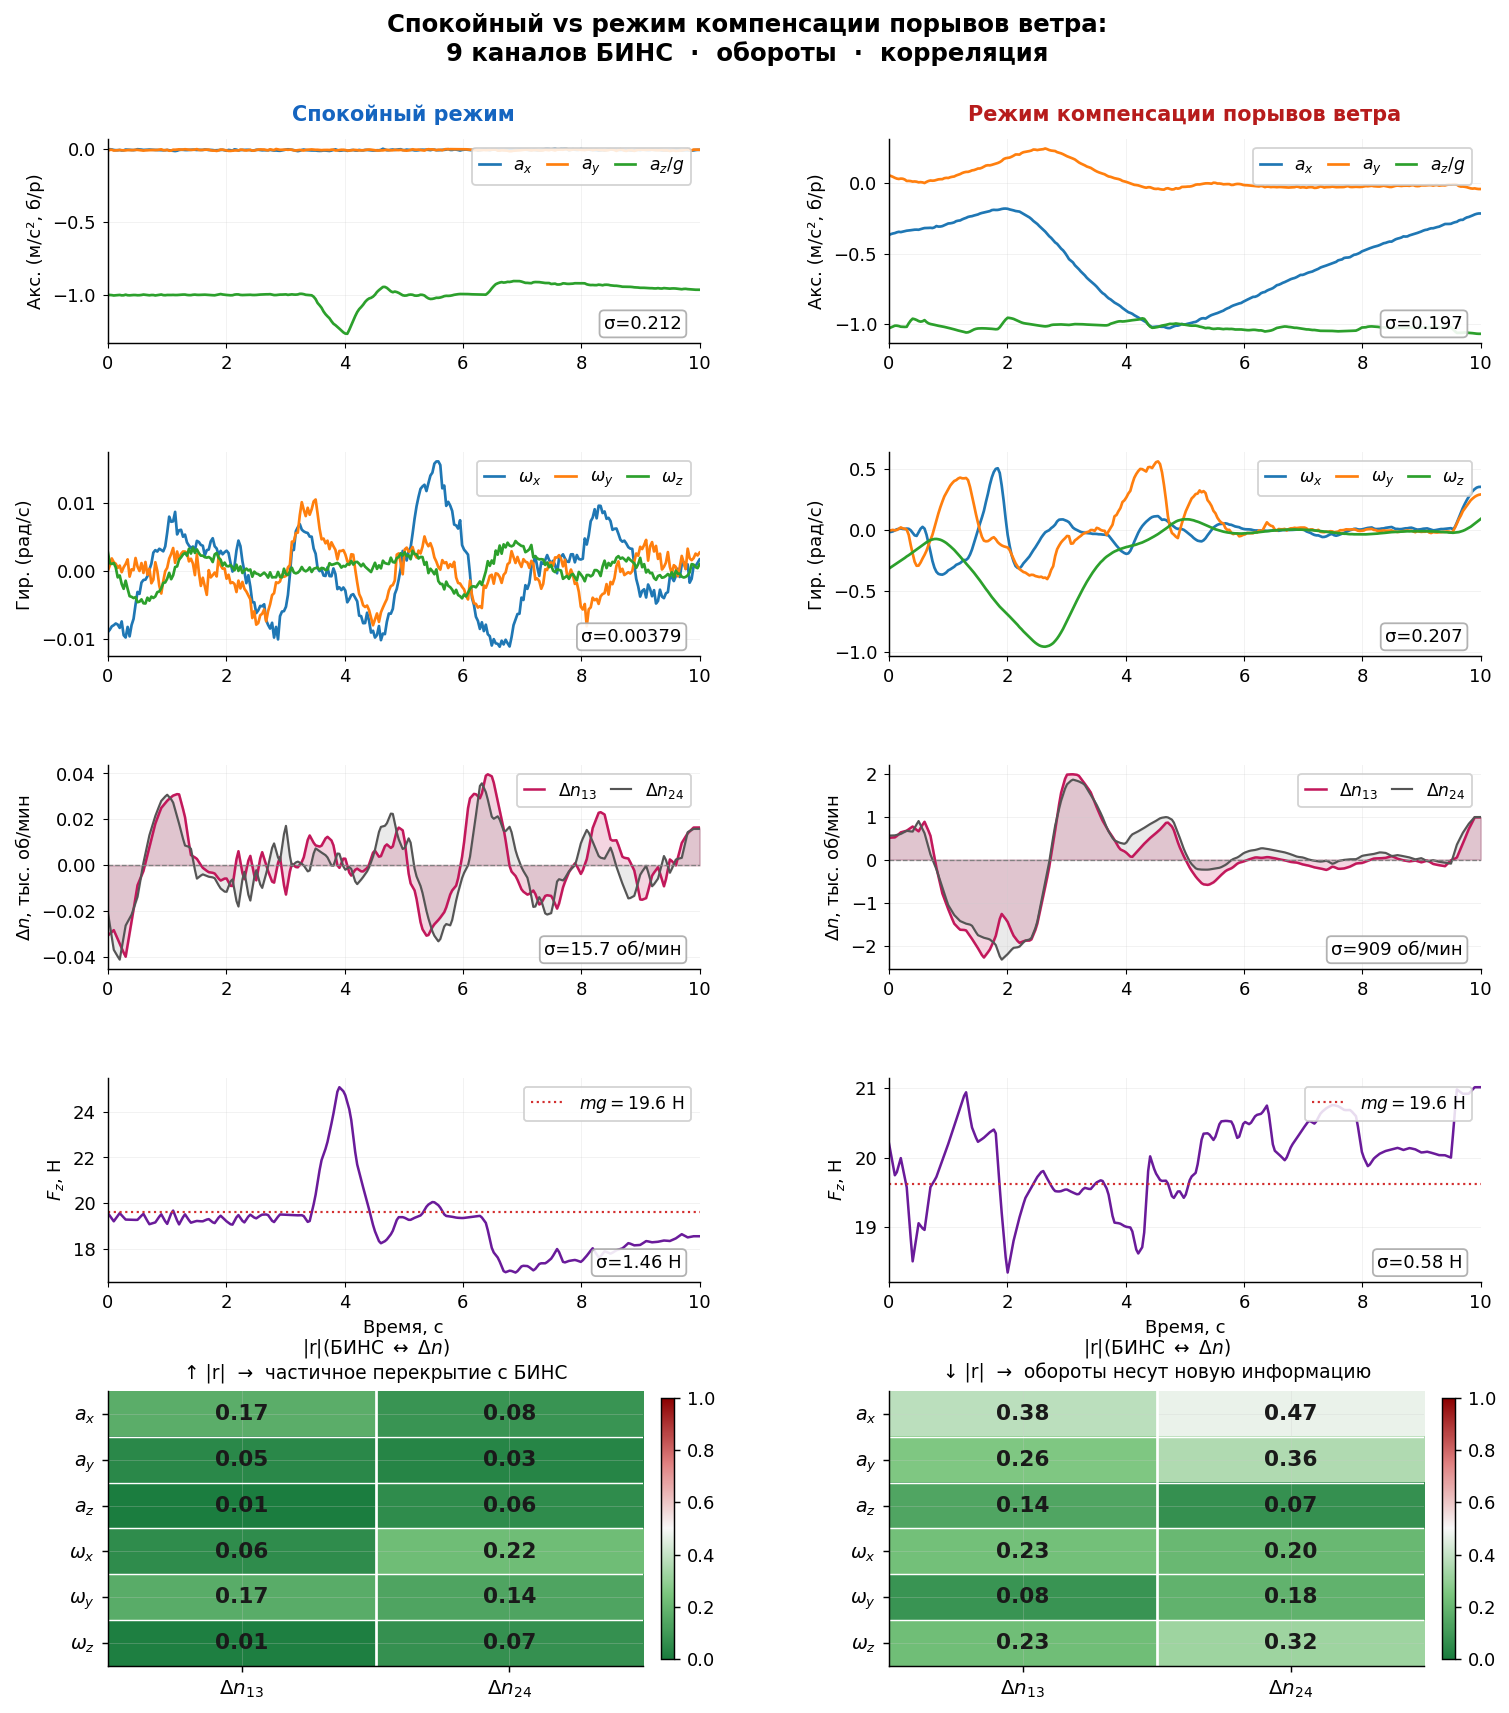
\includegraphics[width=\textwidth]{images/two_regimes_comparison.png}
	\caption{Сравнение спокойного режима и режима компенсации порывов ветра:
		9 каналов БИНС, обороты несущих винтов и корреляция между ними.}
	\label{fig:two_regimes}
\end{figure}

\begin{table}[htbp]
	\centering
	\caption{Сравнение спокойного режима и режима компенсации порывов ветра}
	\label{tab:two_regimes}
	\begin{tabular}{|l|c|c|}
		\hline
		\multirow{2}{*}{Показатель} & \multicolumn{2}{c|}{Режим} \\
		\cline{2-3}
		& Спокойный & Компенсация порывов ветра \\
		\hline
		$\sigma(\Delta n_{13})$, об/мин & 16 & 909 \\
		\hline
		$\sigma(a_z)$, м/с$^2$ & 0{,}212 & 0{,}197 \\
		\hline
		$\sigma(F_z)$, Н & 1{,}46 & 0{,}581 \\
		\hline
		Ср. $|r|$(БИНС, $\Delta n$) & 0{,}08 & 0{,}24 \\
		\hline
	\end{tabular}
\end{table}

Анализ таблицы~\ref{tab:two_regimes} позволяет сформулировать три вывода,
непосредственно определяющих идею предлагаемого метода.


Во-первых, дисперсия вертикального ускорения БИНС~$\sigma(a_z)$ практически одинакова
в обоих режимах (0{,}212 против 0{,}197~м/с$^2$): суммарная тяга остаётся
вблизи~$mg$, и БИНС не фиксирует дифференциальных изменений тяги между
роторами, что соответствует теоретическому выводу из
уравнения~\eqref{eq:trans_dyn}.
Во-вторых, дисперсия оборотов $\sigma(\Delta n_{13})$ возрастает в режиме компенсации
порывов ветра в~57~раз.
Согласно закону~\eqref{eq:thrust}, это показывает значительную временну́ю
изменчивость управляющих сил и моментов, недоступную БИНС.
Именно эта изменчивость порождает повышенный контраст обучающего сигнала
при дообучении нейронной сети с динамическим функционалом потерь.
В третьих, средний~$|r|$ в режиме компенсации порывов ветра составляет лишь 0{,}24,
то есть остаётся низким, несмотря на 57-кратный рост дисперсии оборотов.
Это означает, что в агрессивном режиме сигнал оборотов несёт принципиально
новую, линейно независимую от БИНС информацию об управляющих воздействиях.
Следовательно, регуляризатор на основе телеметрии оборотов не дублирует
информацию, уже содержащуюся в данных БИНС, а добавляет независимый
физически обоснованный надзорный сигнал именно в тех условиях, где
переобучение на малых данных наиболее вероятно.

\subsection{Обзор релевантной литературы}

Дополнительное обоснование дают современные исследования гибридного моделирования и оценки состояния.

Работа NeuroBEM \cite{neurobem2021} представляет гибридную аэродинамическую модель квадрокоптера, сочетающую теорию элемента лопасти (BEM) с нейросетевыми коррекциями. Авторы показывают, что зависимость коэффициентов тяги и момента от относительной скорости набегающего потока делает простую квадратичную модель недостаточной в динамических режимах и при ветровых возмущениях. Измерения оборотов винтов (или команд актуаторов) позволяют значительно точнее оценивать текущие силы и моменты, что напрямую улучшает качество оценки состояния и снижает дрейф.

В исследовании actuator-informed моделей оценки состояния \cite{actuator_informed2022} продемонстрировано, что включение телеметрии оборотов и моментов двигателей в гибридную архитектуру позволяет существенно снизить ошибку инерциальной оценки в условиях внешних возмущений и неопределённости параметров платформы. Авторы отмечают, что сигналы актуаторов обеспечивают дополнительный физический supervision, особенно эффективный при смене динамического режима.

Статья \cite{ssm_actuator2025} посвящена применению последовательностных моделей с селективными пространствами состояний для задач инерциальной навигации с использованием сигналов актуаторов. Показано, что actuator-informed подходы обеспечивают лучшее обобщение при ограниченном объёме данных и при дообучении на новых сценариях — именно та ситуация, которая возникает при адаптации модели к новому промышленному объекту.

Реальный датасет AI-IO \cite{aiio2026} содержит синхронизированные записи IMU и измерений оборотов роторов, полученные на реальном квадрокоптере. Авторы экспериментально подтверждают, что наличие RPM-сигнала позволяет значительно повысить точность одометрии и оценки состояния по сравнению с чисто IMU-based методами в реальных условиях эксплуатации, включая режимы с ветровыми возмущениями.

Наконец, работа по hybrid aerodynamic wind-aware моделям \cite{hawad2023} убедительно показывает, что учёт телеметрии актуаторов критически важен для точной компенсации ветровых возмущений и поддержания физической согласованности модели при резких манёврах. Авторы подчёркивают, что без сигналов оборотов винтов гибридные модели теряют значительную часть своей регуляризационной способности в агрессивных режимах.


\section{Предлагаемая нейронная сеть}
\label{sec:arch}
На основании проведённого анализа установлено,
что сигнал оборотов несущих винтов несёт информацию об управляющих воздействиях,
недоступную БИНС в режиме компенсации порывов ветра, и обеспечивает повышенный
контраст обучающего сигнала при дообучении на малых данных именно в агрессивном
динамическом режиме.

Архитектура предлагаемой нейронной сети состоит из следующих блоков:
входной вектор признаков, кодировщик на основе пространственно-временной
модели состояния (блок линейной проекции, входной блок линейной нормализации,
3 слоя пространственно-временной модели~\cite{Gu2024}, выходной блок линейной
нормализации), выходной вектор признаков.

Входной вектор $\mathbf{x}_t \in \mathbb{R}^{17}$ на каждом временном
шаге~$t$ определяется следующим набором данных:
\begin{equation}
	\mathbf{x}_t = \bigl[
	\mathbf{a}_t,\,\boldsymbol{\omega}_t,\,
	\boldsymbol{\Phi}_t,\;
	\mathbf{p}^{gps}_t,\;
	\mathbf{n_t},\;
	m_t
	\bigr],
	\label{eq:input}
\end{equation}
где $\mathbf{a}_t = [a_x,a_y,a_z]^{\mathrm{T}}$ --- линейное ускорение БИНС;
$\boldsymbol{\omega}_t = [\omega_x,\omega_y,\omega_z]^{\mathrm{T}}$ ---
угловая скорость; $\boldsymbol{\Phi}_t = [\phi,\theta,\psi]^{\mathrm{T}}$ ---
углы ориентации; $\mathbf{p}^{gps}_t$ --- псевдопозиция ГНСС (при потере
сигнала обнуляется); $\mathbf{n}_t = [n_1,n_2,n_3,n_4]^{\mathrm{T}}$ ---
обороты четырёх роторов; $m_t \in \{0,1\}$ --- маска доступности ГНСС.

Выходной вектор $\hat{\mathbf{y}}_t \in \mathbb{R}^{14}$ формируется
конкатенацией четырёх групп предсказаний, извлечённых из скрытого
представления $\mathbf{H}$ линейными проекциями:
\begin{equation}
	\hat{\mathbf{y}}_t = \bigl[
	\hat{\mathbf{v}}_t,\;
	\hat{\mathbf{q}}_t,\;
	\hat{\mathbf{a}}_t,\;
	\boldsymbol{\tau}
	\bigr],
	\label{eq:output}
\end{equation}
где $\hat{\mathbf{v}}_t \in \mathbb{R}^3$ --- предсказанная линейная скорость;
$\hat{\mathbf{q}}_t \in [-1,1]^4$ --- нормированный кватернион ориентации;
$\hat{\mathbf{a}}_t \in \mathbb{R}^3$ --- линейное ускорение в связанной
системе координат; $\boldsymbol{\tau}_{\mathrm int,t} \in \mathbb{R}^4$ ---
промежуточное представление управляющих моментов, используемое
в динамическом функционале потерь.

Из скрытого представления $\mathbf{H}$ компоненты выходного вектора
извлекаются посредством линейных проекций:
\begin{align}
	\hat{\mathbf{v}} &= \mathbf{H}\mathbf{W}_v \in \mathbb{R}^{T\times 3},
	\label{eq:vel} \\
	\hat{\mathbf{q}} &= \frac{\mathbf{H}\mathbf{W}_q}
	{\|\mathbf{H}\mathbf{W}_q\|},\quad
	\hat{\mathbf{q}} \in [-1,1]^{T\times 4},
	\label{eq:quat} \\
	\hat{\mathbf{a}} &= \mathbf{H}\mathbf{W}_a \in \mathbb{R}^{T\times 3},
	\label{eq:accel} \\
	\boldsymbol{\tau}_{\mathrm int} &= \mathbf{H}\mathbf{W}_\tau
	\in \mathbb{R}^{T\times 4}.
	\label{eq:torque}
\end{align}
Нормировка кватерниона гарантирует принадлежность многообразию~$S^3$.

Ключевое отличие предлагаемой нейронной сети от остальных моделей заключается
в функции потерь, связывающей предсказания модели с законами динамики
квадрокоптера.


Итоговая функция потерь:
\begin{equation}
	\mathcal{L}_{DF} = \lambda_1 \mathcal{L}_{traj}
	+ \lambda_2 \left\|\frac{\boldsymbol{\varepsilon}_F}{mg}\right\|^2
	+ \lambda_3 \left\|\frac{\boldsymbol{\varepsilon}_\tau}{\sigma_\tau}\right\|^2,
	\label{eq:loss_df}
\end{equation}
где $\|\cdot\|^2$ обозначает среднеквадратическую ошибку по компонентам вектора;
$mg$ --- нормировочный множитель, приводящий невязку тяги к безразмерному виду;
$\sigma_\tau$ --- стандартное отклонение момента на текущем батче.
Весовые коэффициенты $\lambda_1 = 1{,}0$, $\lambda_2 = \lambda_3 = 3{\times}10^{-4}$
подобраны на валидационной выборке датасета~A из условия соизмеримости слагаемых:
физические штрафные члены вносят регуляризующий вклад, не подавляя основной
траекторный сигнал на начальных эпохах обучения.
Базовая нейронная сеть использует только $\mathcal{L}_{traj}$
(то есть $\lambda_2=\lambda_3=0$);
обобщённая нейронная сеть включает регуляризатор без прямой зависимости от~$n_i$.

При высокой дисперсии $n_i$ значение $F_z(t)$ значительно изменяется во
времени, а штрафные слагаемые $\|\varepsilon_F\|^2$ и $\|\varepsilon_\tau\|^2$
создают повышенный контраст обучающего сигнала при дообучении, ограничивая
пространство допустимых весов модели именно в тех режимах, где переобучение
на малых данных наиболее вероятно.

Траекторная составляющая функции потерь $\mathcal{L}_{traj}$ включает
три слагаемых:
\begin{equation}
	\mathcal{L}_{traj} =
	\underbrace{\|\hat{\mathbf{v}} - \mathbf{v}\|^2}_{\text{ошибка скорости}}
	+ 0{,}5\,
	\underbrace{\mathcal{L}_{q}(\hat{q},\, q)}_{\text{ошибка ориентации}}
	+ \lambda_{pos}\,
	\underbrace{\|\hat{p} - p\|^2}_{\text{ошибка позиции}},
	\label{eq:Ltraj}
\end{equation}
где $\hat{\mathbf{v}}, \mathbf{v}$ --- предсказанная и истинная скорость;
$\hat{q}, q$ --- предсказанный и истинный кватернион ориентации;
$\hat{p}, p$ --- предсказанная и истинная траектория, восстановленная
интегрированием скорости методом Эйлера;
$\mathcal{L}_{q} = \|\hat{q} - q\|^2 + 0{,}5\,(\|\hat{q}\| - 1)^2$ ---
функция потерь по кватерниону, включающая штраф за отклонение от единичной нормы;
$\lambda_{pos} = 0{,}15$ --- весовой коэффициент позиционного слагаемого.

Общая схема предлагаемой нейронной сети представлена на рисунке~\ref{fig:arch}.

\begin{figure}[htbp]
	\centering
	\includegraphics[width=\textwidth]{images/fig-arch.png}
	\caption{Архитектура ФИ НС-ПСПС.}
	\label{fig:arch}
\end{figure}


